% ------------------------------------------------------------
% LaTeX Template für die DHBW zum Schnellstart!
% Original: https://github.wdf.sap.corp/vtgermany/LaTeX-Template-DHBW
% ------------------------------------------------------------
% ---- Präambel mit Angaben zum Dokument
\documentclass[
	fontsize=12pt,           % Leitlinien sprechen von Schriftgröße 12.
	paper=A4,
	twoside=false,
	listof=totoc,            % Tabellen- und Abbildungsverzeichnis ins Inhaltsverzeichnis
	bibliography=totoc,      % Literaturverzeichnis ins Inhaltsverzeichnis aufnehmen
	titlepage,               % Titlepage-Umgebung anstatt \maketitle
	headsepline,             % horizontale Linie unter Kolumnentitel
	abstract,              % Überschrift einschalten, Abstract muss in {abstract}-Umgebung stehen
]{scrreprt}                  % Verwendung von KOMA-Report
\usepackage[utf8]{inputenc}  % UTF8 Encoding einschalten
\usepackage[english]{babel}  % Neue deutsche Rechtschreibung
\usepackage[T1]{fontenc}     % Ausgabe von westeuropäischen Zeichen (auch Umlaute)
\usepackage{microtype}       % Trennung von Wörtern wird besser umgesetzt
\usepackage{lmodern}         % Nicht-gerasterte Schriftarten (bei MikTeX erforderlich)
\usepackage{graphicx}        % Einbinden von Grafiken erlauben
\usepackage{wrapfig}         % Grafiken fließend im Text
\usepackage{setspace}        % Zeilenabstand \singlespacing, \onehalfspaceing, \doublespacing
\usepackage[
	%showframe,                % Ränder anzeigen lassen
	left=2.7cm, right=2.5cm,
	top=2.5cm,  bottom=2.5cm,
	includeheadfoot
]{geometry}                      % Seitenlayout einstellen
\usepackage{scrlayer-scrpage}    % Gestaltung von Fuß- und Kopfzeilen
\usepackage{acronym}             % Abkürzungen, Abkürzungsverzeichnis
\usepackage{titletoc}            % Anpassungen am Inhaltsverzeichnis
\contentsmargin{0.75cm}          % Abstand im Inhaltsverzeichnis zw. Punkt und Seitenzahl
\usepackage[                     % Klickbare Links (enth. auch "nameref", "url" Package)
  hidelinks,                     % Blende die "URL Boxen" aus.
  breaklinks=true                % Breche zu lange URLs am Zeilenende um
]{hyperref}
\usepackage[hypcap=true]{caption}% Anker Anpassung für Referenzen
\urlstyle{same}                  % Aktuelle Schrift auch für URLs
% Anpassung von autoref für Gleichungen (ergänzt runde Klammern) und Algorithm.
% Anstatt "Listing" kann auch z.B. "Code-Ausschnitt" verwendet werden. Dies sollte
% jedoch synchron gehalten werden mit \lstlistingname (siehe weiter unten).
\addto\extrasenglish{%
	\def\equationautorefname~#1\null{Equation~(#1)\null}
	\def\lstnumberautorefname{Line}
	\def\lstlistingautorefname{Code listing}
	\def\algorithmautorefname{Algorithm}
	% Damit einheitlich "Abschnitt 1.2[.3]" verwendet wird und nicht "Unterabschnitt 1.2.3"
	% \def\subsectionautorefname{Abschnitt}
}

% ---- Abstand verkleinern von der Überschrift 
\renewcommand*{\chapterheadstartvskip}{\vspace*{.5\baselineskip}}

% Hierdurch werden Schusterjungen und Hurenkinder vermieden, d.h. einzelne Wörter
% auf der nächsten Seite oder in einer einzigen Zeile.
% LaTeX kann diese dennoch erzeugen, falls das Layout ansonsten nicht umsetzbar ist.
% Diese Werte sind aber gute Startwerte.
\widowpenalty10000
\clubpenalty10000

% ---- Für das Quellenverzeichnis
\usepackage[
	backend = biber,                % Verweis auf biber
	language = auto,
	style = numeric,                % Nummerierung der Quellen mit Zahlen
	sorting = none,                 % none = Sortierung nach der Erscheinung im Dokument
	sortcites = true,               % Sortiert die Quellen innerhalb eines cite-Befehls
	block = space,                  % Extra Leerzeichen zwischen Blocks
	hyperref = true,                % Links sind klickbar auch in der Quelle
	%backref = true,                % Referenz, auf den Text an die zitierte Stelle
	bibencoding = auto,
	giveninits = true,              % Vornamen werden abgekürzt
	doi=false,                      % DOI nicht anzeigen
	isbn=false,                     % ISBN nicht anzeigen
    alldates=long                  % Datum immer als DD.MM.YYYY anzeigen
]{biblatex}
\addbibresource{Inhalt/literatur.bib}
\setcounter{biburlnumpenalty}{3000}     % Umbruchgrenze für Zahlen
\setcounter{biburlucpenalty}{6000}      % Umbruchgrenze für Großbuchstaben
\setcounter{biburllcpenalty}{9000}      % Umbruchgrenze für Kleinbuchstaben
\DeclareNameAlias{default}{family-given}  % Nachname vor dem Vornamen
\AtBeginBibliography{\renewcommand{\multinamedelim}{\addslash\space
}\renewcommand{\finalnamedelim}{\multinamedelim}}  % Schrägstrich zwischen den Autorennamen
%\DefineBibliographyStrings{german}{
%  urlseen = {Seen:},                      % Ändern des Titels von "besucht am"
%}
\usepackage[babel,german=quotes]{csquotes}         % Deutsche Anführungszeichen + Zitate


% ---- Für Mathevorlage
\usepackage{amsmath}    % Erweiterung vom Mathe-Satz
\usepackage{amssymb}    % Lädt amsfonts und weitere Symbole
\usepackage{MnSymbol}   % Für Symbole, die in amssymb nicht enthalten sind.


% ---- Für Quellcodevorlage
\usepackage{scrhack}                    % Hack zur Verw. von listings in KOMA-Script
\usepackage{listings}                   % Darstellung von Quellcode
\usepackage{xcolor}                     % Einfache Verwendung von Farben
% -- Eigene Farben für den Quellcode
\definecolor{JavaLila}{rgb}{0.4,0.1,0.4}
\definecolor{JavaGruen}{rgb}{0.3,0.5,0.4}
\definecolor{JavaBlau}{rgb}{0.0,0.0,1.0}
\definecolor{greenString}{HTML}{13752f}
\definecolor{ABAPKeywordsBlue}{HTML}{6000ff}
\definecolor{ABAPCommentGrey}{HTML}{808080}
\definecolor{ABAPStringGreen}{HTML}{4da619}
\definecolor{PyKeywordsBlue}{HTML}{0000AC}
\definecolor{PyCommentGrey}{HTML}{808080}
\definecolor{PyStringGreen}{HTML}{008080}
% -- Farben für ABAP CDS
\definecolor{CDSString}{HTML}{FF8C00}
\definecolor{CDSKeywords}{HTML}{6000ff}
\definecolor{CDSAnnotation}{HTML}{00BFFF}
\definecolor{CDSComment}{HTML}{808080}
\definecolor{CDSFunc}{HTML}{FF0000}

% -- Default Listing-Styles

\lstset{
	% Das Paket "listings" kann kein UTF-8. Deswegen werden hier 
	% die häufigsten Zeichen definiert (ä,ö,ü,...)
	literate=%
		{á}{{\'a}}1 {é}{{\'e}}1 {í}{{\'i}}1 {ó}{{\'o}}1 {ú}{{\'u}}1
		{Á}{{\'A}}1 {É}{{\'E}}1 {Í}{{\'I}}1 {Ó}{{\'O}}1 {Ú}{{\'U}}1
		{à}{{\`a}}1 {è}{{\`e}}1 {ì}{{\`i}}1 {ò}{{\`o}}1 {ù}{{\`u}}1
		{À}{{\`A}}1 {È}{{\'E}}1 {Ì}{{\`I}}1 {Ò}{{\`O}}1 {Ù}{{\`U}}1
		{ä}{{\"a}}1 {ë}{{\"e}}1 {ï}{{\"i}}1 {ö}{{\"o}}1 {ü}{{\"u}}1
		{Ä}{{\"A}}1 {Ë}{{\"E}}1 {Ï}{{\"I}}1 {Ö}{{\"O}}1 {Ü}{{\"U}}1
		{â}{{\^a}}1 {ê}{{\^e}}1 {î}{{\^i}}1 {ô}{{\^o}}1 {û}{{\^u}}1
		{Â}{{\^A}}1 {Ê}{{\^E}}1 {Î}{{\^I}}1 {Ô}{{\^O}}1 {Û}{{\^U}}1
		{œ}{{\oe}}1 {Œ}{{\OE}}1 {æ}{{\ae}}1 {Æ}{{\AE}}1 {ß}{{\ss}}1
		{ű}{{\H{u}}}1 {Ű}{{\H{U}}}1 {ő}{{\H{o}}}1 {Ő}{{\H{O}}}1
		{ç}{{\c c}}1 {Ç}{{\c C}}1 {ø}{{\o}}1 {å}{{\r a}}1 {Å}{{\r A}}1
		{€}{{\euro}}1 {£}{{\pounds}}1 {«}{{\guillemotleft}}1
		{»}{{\guillemotright}}1 {ñ}{{\~n}}1 {Ñ}{{\~N}}1 {¿}{{?`}}1,
	breaklines=true,        % Breche lange Zeilen um 
	breakatwhitespace=true, % Wenn möglich, bei Leerzeichen umbrechen
	% Symbol für Zeilenumbruch einfügen
	prebreak=\raisebox{0ex}[0ex][0ex]{\ensuremath{\rhookswarrow}},
	postbreak=\raisebox{0ex}[0ex][0ex]{\ensuremath{\rcurvearrowse\space}},
	tabsize=4,                                 % Setze die Breite eines Tabs
	basicstyle=\ttfamily\small,                % Grundsätzlicher Schriftstyle
	columns=fixed,                             % Besseres Schriftbild
	numbers=left,                              % Nummerierung der Zeilen
	%frame=single,                             % Umrandung des Codes
	showstringspaces=false,                    % Keine Leerzeichen hervorheben
	keywordstyle=\color{blue},
	ndkeywordstyle=\bfseries\color{darkgray},
	identifierstyle=\color{black},
	commentstyle=\itshape\color{JavaGruen},   % Kommentare in eigener Farbe
	stringstyle=\color{JavaBlau},             % Strings in eigener Farbe,
	captionpos=b,                             % Bild*unter*schrift
	xleftmargin=5.0ex
}

% ---- Eigener JAVA-Style für den Quellcode
\renewcommand{\ttdefault}{pcr}               % Schriftart, welche auch fett beinhaltet
\lstdefinestyle{EigenerJavaStyle}{
	language=Java,                             % Syntax Highlighting für Java
	%frame=single,                             % Umrandung des Codes
	keywordstyle=\bfseries\color{JavaLila},    % Keywords in eigener Farbe und fett
	commentstyle=\itshape\color{JavaGruen},    % Kommentare in eigener Farbe und italic
	stringstyle=\color{JavaBlau}               % Strings in eigener Farbe
}

% ---- Eigener ABAP-Style für den Quellcode
\renewcommand{\ttdefault}{pcr}
\lstdefinestyle{EigenerABAPStyle}{
	language=[R/3 6.10]ABAP,
	morestring=[b]\|,                          % Für Pipe-Strings
	morestring=[b]\`,                          % für Backtick-Strings
	keywordstyle=\bfseries\color{ABAPKeywordsBlue},
	commentstyle=\itshape\color{ABAPCommentGrey},
	stringstyle=\color{ABAPStringGreen},
	tabsize=2,
	morekeywords={
		types,
		@data,
		as,
		lower,
		start,
		selection,
		order,
		by,
		inner,
		join,
		key,
		end,
		cast
	}
}

% ---- Eigener Python-Style für den Quellcode
\renewcommand{\ttdefault}{pcr}
\lstdefinestyle{EigenerPythonStyle}{
	language=Python,
	columns=flexible,
	keywordstyle=\bfseries\color{PyKeywordsBlue},
	commentstyle=\itshape\color{PyCommentGrey},
	stringstyle=\color{PyStringGreen}
}

% ---- Eigener Go-Style für den Quellcode
\renewcommand{\ttdefault}{pcr}
\lstdefinestyle{EigenerGoStyle}{
	language=Go,
	columns=flexible,
	keywordstyle=\bfseries\color{JavaLila},    % Keywords in eigener Farbe und fett
	commentstyle=\itshape\color{JavaGruen},    % Kommentare in eigener Farbe und italic
	stringstyle=\color{greenString}               % Strings in eigener Farbe
}

% ---- Eigener Json-Style für den Quellcode
\renewcommand{\ttdefault}{pcr}
\lstdefinestyle{EigenerJsonStyle}{
	language=Go,
	columns=flexible,
	keywordstyle=\bfseries\color{JavaLila},    % Keywords in eigener Farbe und fett
	commentstyle=\itshape\color{JavaGruen},    % Kommentare in eigener Farbe und italic
	stringstyle=\color{greenString}               % Strings in eigener Farbe
}

%----- ABAP-CDS-View language
\lstdefinelanguage{ABAPCDS}{
	sensitive=false,
	%Keywords
	morekeywords={define,
		view,
		as,
		select,
		from,
		inner,
		join,
		on,
		key,
		case,
		when,
		then,
		else,
		end,
		true,
		false,
		cast,
		where,
		and,
		distinct,
		group,
		by,
		having,
		min,
		sum,
		max,
		count,
		avg
	},
	%Methoden
	morekeywords=[2]{
		div,
		currency\_conversion,
		dats\_days\_between,
		concat\_with\_space,
		dats\_add_days,
		dats\_is\_valid,
		dats\_add\_months,
		unit\_conversion,
		division,
		mod,
		abs,
		floor,
		ceil,
		round,
		concat,
		replace,
		substring,
		left,
		right,
		length
	},
	morecomment=[s][\color{CDSAnnotation}]{@}{:},
	morecomment=[l][\itshape\color{CDSComment}]{//},
	morecomment=[s][\itshape\color{CDSComment}]{/*}{*/},
	morestring=[b][\color{CDSString}]',
	keywordstyle=\bfseries\color{CDSKeywords},
	keywordstyle=[2]\color{CDSFunc}
}

  % Weitere Details sind ausgelagert

\usepackage{algorithm}                  % Für Algorithmen-Umgebung (ähnlich wie lstlistings Umgebung)
\usepackage{algpseudocode}              % Für Pseudocode. Füge "[noend]" hinzu, wenn du kein "endif",
                                        % etc. haben willst.

\makeatletter                           % Sorgt dafür, dass man @ in Namen verwenden kann.
                                        % Ansonsten gibt es in der nächsten Zeile einen Compilefehler.
\renewcommand{\ALG@name}{Algorithm}   % Umbenennen von "Algorithm" im Header der Listings.
\makeatother                            % Zeichen wieder zurücksetzen
\renewcommand{\lstlistingname}{Code listing} % Erlaubt das Umbenennen von "Listing" in anderen Titel.

% ---- Tabellen
\usepackage{booktabs}  % Für schönere Tabellen. Enthält neue Befehle wie \midrule
\usepackage{multirow}  % Mehrzeilige Tabellen
\usepackage{siunitx}   % Für SI Einheiten und das Ausrichten Nachkommastellen
\sisetup{locale=DE, range-phrase={~bis~}, output-decimal-marker={,}} % Damit ein Komma und kein Punkt verwendet wird.
\usepackage{xfrac} % Für siunitx Option "fraction-function=\sfrac"

% ---- Für Definitionsboxen in der Einleitung
\usepackage{amsthm}                     % Liefert die Grundlagen für Theoreme
\usepackage[framemethod=tikz]{mdframed} % Boxen für die Umrandung
% ---- Definition für Highlight Boxen

% ---- Grundsätzliche Definition zum Style
\newtheoremstyle{defi}
  {\topsep}         % Abstand oben
  {\topsep}         % Abstand unten
  {\normalfont}     % Schrift des Bodys
  {0pt}             % Einschub der ersten Zeile
  {\bfseries}       % Darstellung von der Schrift in der Überschrift
  {:}               % Trennzeichen zwischen Überschrift und Body
  {.5em}            % Abstand nach dem Trennzeichen zum Body Text
  {\thmname{#3}}    % Name in eckigen Klammern
\theoremstyle{defi}

% ------ Definition zum Strich vor eines Texts
\newmdtheoremenv[
  hidealllines = true,       % Rahmen komplett ausblenden
  leftline = true,           % Linie links einschalten
  innertopmargin = 0pt,      % Abstand oben
  innerbottommargin = 4pt,   % Abstand unten
  innerrightmargin = 0pt,    % Abstand rechts
  linewidth = 3pt,           % Linienbreite
  linecolor = gray!40,       % Linienfarbe
]{defStrich}{Definition}     % Name der des formats "defStrich"

% ------ Definition zum Eck-Kasten um einen Text
\newmdtheoremenv[
  hidealllines = true,
  innertopmargin = 6pt,
  linecolor = gray!40,
  singleextra={              % Eck-Markierungen für die Definition
    \draw[line width=3pt,gray!50,line cap=rect] (O|-P) -- +(1cm,0pt);
    \draw[line width=3pt,gray!50,line cap=rect] (O|-P) -- +(0pt,-1cm);
    \draw[line width=3pt,gray!50,line cap=rect] (O-|P) -- +(-1cm,0pt);
    \draw[line width=3pt,gray!50,line cap=rect] (O-|P) -- +(0pt,1cm);
  }
]{defEckKasten}{Definition}  % Name der des formats "defEckKasten"  % Weitere Details sind ausgelagert

% ---- Für Todo Notes
\usepackage{todonotes}
\setlength {\marginparwidth }{2cm}      % Abstand für Todo Notizen

% ---- Für PDFs-Anhängen
\usepackage{pdfpages}
 

% ---- Elektronische Version oder Gedruckte Version?
% ---- Unterschied: Die elektronische Version enthält keinen Platzhalter für die Unterschrift
\usepackage{ifthen}
\usepackage{algpseudocode}
\usepackage{multirow}
\usepackage{subcaption} 
\usepackage{tikz}
\usepackage{rotating}
\usepackage{float}
\usepackage{afterpage}
\usepackage{enumitem}
\newboolean{e-Abgabe}
\setboolean{e-Abgabe}{true}    % false=gedruckte Fassung

% ---- Persönlichen Daten:
\newcommand{\titel}{Advanced Software Engineering}
\newcommand{\titelheader}{ASE}
\newcommand{\arbeit}{Projektdokumentation}
\newcommand{\studiengang}{Informatik (Computer Science)}
\newcommand{\studienjahr}{2022}
\newcommand{\autor}{Lukas Rapp and Simon Reichle}
\newcommand{\autorReverse}{Rapp, Lukas}
\newcommand{\verfassungsort}{Karlsruhe}
\newcommand{\matrikelnr}{7602924, 7400045}
\newcommand{\kurs}{TINF20B2}
\newcommand{\bearbeitungsmonat}{Oktober 2022 - May 2023}
\newcommand{\abgabe}{May 28th, 2023}
\newcommand{\bearbeitungszeitraum}{04.10.2022 - 28.05.2023}
\newcommand{\firmaName}{SAP SE}
\newcommand{\firmaStrasse}{Dietmar-Hopp-Allee 16}
\newcommand{\firmaPlz}{69190 Walldorf, Germany}
% \newcommand{\betreuerFirma}{-}
\newcommand{\betreuerDhbw}{Dr. Lars Briem}

% ---- Metainformation für das PDF Dokument
\hypersetup{
	pdftitle    = {\titel},
	pdfsubject  = {\arbeit},
	pdfauthor   = {\autor},
	%pdfkeywords = {Keywords angeben},
	pdfcreator  = {LaTeX},
	%pdfproducer = {in der Regel pdfTeX}
}

% ---- Definition der Kopf- und Fußzeilen
\clearscrheadfoot                               % Löschen von LaTeX Standard
\automark[section]{chapter}                     % Füllen von section und chapter
\renewcommand*{\chaptermarkformat}{}            % Entfernt die Kapitelnummer
\renewcommand*{\sectionmarkformat}{}            % Entfernt die Sectionnummer
% Angaben [für "plain"]{für "scrheadings"}
\ihead[]{\titelheader}                          % Kopfzeile links
\chead[]{}                                      % Kopfzeile mitte
\ohead[]{\rightmark}                            % Kopfzeile rechts
\ifoot[]{}                                      % Fußzeile links
\cfoot*{\sffamily\pagemark}                     % Fußzeile mitte
\ofoot[]{}                                      % Fußzeile rechts
\KOMAoptions{
   headsepline = 0.2pt,                         % Liniendicke Kopfzeile
   footsepline = false                          % Liniendicke Fußzeile
}

% ---- Hilfreiches
\newcommand{\zB}{z.\,B. }   % "z.B." mit kleinem Leeraum dazwischen (ohne wäre nicht korrekt)
\newcommand{\dash}{d.\,h. }

\newcommand{\code}[1]{\texttt{#1}} % Ist einfacher zu schreiben als ständig \texttt und erlaubt
                                   % Änderungen im Nachhinein, wenn man z.B. Inline-Code anders stylen möchte.

% ---- Silbentrennung (falls LaTeX defaults falsch / nicht gewünscht sind)
\hyphenation{HANA}         % anstatt HA-NA
\hyphenation{Graph-Script} % anstatt GraphS-cript

% ---- Watermark/Wasserzeichen
%% ---- Für Watermarks
\usepackage{background}
\usepackage{eso-pic}

\makeatletter
\let \AddEverypageHook \AddToShipoutPictureFG
\renewcommand\AddThispageHook{\AddToShipoutPictureFG*}
\ifbg@some
  \AddThispageHook{}
\else
  \AddEverypageHook{\bg@material}
\fi
\makeatother

\newcommand{\watermark}[3][0.07]{
\backgroundsetup{
  color=#2,
  angle=45,
  opacity=#1,
  contents={\Large{#3}},
}
\SetBgScale{5.8}
}

\newcommand{\SetWatermarkSize}[1]{\SetBgScale{#1}}
 % Auskommentieren wenn nicht erwünscht
%\watermark{gray}{\textbf{DRAFT}}     % Auskommentieren wenn nicht erwünscht. Nimmt optional die opacity/Deckraft z.B. \watermark[0.1]{green}{text} für 10% Deckkraft
%\SetWatermarkSize{8} % Optional. Standard ist 5.8. 

% ---- Beginn des Dokuments
\begin{document}
\setlength{\parindent}{0pt}              % Keine Paragraphen Einrückung.
                                         % Dafür haben wir den Abstand zwischen den Paragraphen.
\setcounter{secnumdepth}{2}              % Nummerierungstiefe fürs Inhaltsverzeichnis
\setcounter{tocdepth}{1}                 % Tiefe des Inhaltsverzeichnisses. Ggf. so anpassen,
                                         % dass das Verzeichnis auf eine Seite passt.
%\sffamily                                % Serifenlose Schrift verwenden.

% ---- Vorspann
% ------ Titelseite
\singlespacing
\thispagestyle{empty}
\begin{titlepage}
\enlargethispage{4cm}

\begin{figure}          
	% \vspace*{-5mm} % in case the title is too long
	\begin{minipage}{0.49\textwidth}
		\flushleft
		
\includegraphics[height=2.5cm]{Bilder/Logos/Logo_SAP.pdf} 
	\end{minipage}
	\hfill
	\begin{minipage}{0.49\textwidth}
		\flushright
		
\includegraphics[height=2.5cm]{Bilder/Logos/Logo_DHBW.pdf} 
	\end{minipage}
\end{figure} 
\vspace*{0.1cm}

\begin{center}
	\huge{\textbf{\titel}}\\[1cm]
	\Large{\textbf{\arbeit}}\\[0.5cm]
	\normalsize{for the examination of Bachelor of Science (B.Sc.)}\\[0.2cm]
	\normalsize{in \textbf{\studiengang}}\\[1ex]
	\normalsize{at Duale Hochschule Baden-Württemberg Karlsruhe}\\[0.5cm]
	\normalsize{authored by}\\[1ex] \Large{\textbf{\autor}} \\
\end{center}

\begin{center}
	\vfill
	\begin{tabular}{ll}
		Due date:                     & \abgabe \\[0.2cm]
		Matriculation number, class:            & \matrikelnr , \kurs \\[0.2cm]
		% Supervisor:   & \betreuerFirma \\[0.2cm]
		Period: & \bearbeitungszeitraum \\[0.2cm]
		Inspector at Duale Hochschule: & \betreuerDhbw \\[2cm]
	\end{tabular} 
\end{center}
\end{titlepage}
  % Titelseite
\newcounter{savepage}
\pagenumbering{Roman}                    % Römische Seitenzahlen
\onehalfspacing

% ------ Erklärung, Sperrvermerk, Abstact
% \section*{Blocking Notice}
This document contains confidential data of

\begin{quote}
	\firmaName \\
	\firmaStrasse \\
	\firmaPlz
\end{quote}

\vspace{0.5cm}

The contents of this document shall neither completely nor partially be disclosed to anyone outside of the examination and evaluation process unless an explicit permit of the aforementioned organization exists.


\vspace*{\fill}

\section*{Trademark Notice}

This document contains mentions of company trademarks, products and services including but not limited to the aforementioned organization. These mentions do not constitute the usage of trademarks in a business context and solely serve a scientific purpose. Therefore, for reasons of better readability and accessibility, these trademarks are not marked as such.
%\section*{Declaration of Authorship}
I hereby declare that my \arbeit{} titled:
\begin{quote}
	\textit{\titel}
\end{quote} 
is my own unaided work in compliance with § 5 of \enquote{Studien- und Prüfungsordnung DHBW Technik} (September 29, 2017). All direct or indirect sources used are acknowledged as references.
This paper was not previously presented to another examination board and has not been
published.

\vspace{0.25cm}

I also assure that the electronically entered version matches with the printed version.

\vspace{1cm}

\verfassungsort, \today \\[0.5cm]
\ifthenelse{\boolean{e-Abgabe}}
	
	{_____________________________}
	{\makebox[6cm]{\hrulefill}}\\ 
\autorReverse

\vspace*{\fill}

%\renewcommand{\abstractname}{Abstract} % Veränderter Name für das Abstract
\begin{abstract}
\begin{addmargin}[1.5cm]{1.5cm}        % Erhöhte Ränder, für Abstract Look
\thispagestyle{plain}                  % Seitenzahl auf der Abstract Seite

\begin{center}
\small\textit{- English -}             % Angabe der Sprache für das Abstract
\end{center}

\end{addmargin}
\end{abstract}

%\renewcommand{\abstractname}{Abstract} % Veränderter Name für das Abstract
\begin{abstract}
\begin{addmargin}[1.5cm]{1.5cm}        % Erhöhte Ränder, für Abstract Look
\thispagestyle{plain}                  % Seitenzahl auf der Abstract Seite

\begin{center}
\small\textit{- Deutsch -}             % Angabe der Sprache für das Abstract
\end{center}

\end{addmargin}
\end{abstract}


% ------ Inhaltsverzeichnis
\singlespacing
\tableofcontents

% ------ Verzeichnisse
\renewcommand*{\chapterpagestyle}{plain}
\pagestyle{plain}
%\chapter*{List of Abbreviations}
\addcontentsline{toc}{chapter}{List of Abbreviations} % Hinzufügen zum Inhaltsverzeichnis 

\begin{acronym}[WYSISWG] % längstes Kürzel wird verw. für den Abstand zw. Kürzel u. Text

\end{acronym}

\listoffigures                          % Erzeugen des Abbildungsverzeichnisses 
%\listoftables                          % Erzeugen des Tabellenverzeichnisses
%\renewcommand{\lstlistlistingname}{List of Code Listings}
% \lstlistoflistings                      % Erzeugen des Listenverzeichnisses
\setcounter{savepage}{\value{page}}

% ---- Inhalt der Arbeit
\cleardoublepage
\pagenumbering{arabic}                  % Arabische Seitenzahlen für den Hauptteil
\setlength{\parskip}{0.5\baselineskip}  % Abstand zwischen Absätzen
\rmfamily
\renewcommand*{\chapterpagestyle}{scrheadings}
\pagestyle{scrheadings}
\onehalfspacing

\chapter{Einführung}

\section{Übersicht über die Applikation}
Bei dieser Applikation handelt es sich um einen
\textit{Single Player Dungeon Crawler}, der
\textit{The Binding Of Isaac} in seinen Grundzügen nachempfunden ist.
Der Spieler bewegt sich durch prozedural generierte Level. Dabei kann
er verschiedene Gegenstände einsammeln wie Rüstung (\textit{Armor}),
Waffen (\textit{Weapons}), Münzen (\textit{Coins}) und Herzen
(\textit{Hearts}). Diese Gegenstände sollen ihm dabei helfen zu
überleben. Die Münzen stellen jedoch den Punktestand dar.
Während der Spieler sich durch die Räume bewegt, stößt er
auf eine Palette unterschiedlicher Gegner (\textit{Spider}, 
\textit{Skeleton}, {Zombie}, \textit{Ogre}). Diese besitzen auch
unterschiedliche Fähigkeiten und versuchen den Spieler zu besiegen.
Betritt der Spieler einen Raum, so wird dieser gesperrt, bis er alle
darin befindlichen Gegner besiegt hat. Erst dann öffnen sich die Türen
wieder und der Spieler kann in anliegende Räume laufen.
Stirbt der Spieler dabei, so ist das Spiel zu Ende. Bleibt er am Leben,
hangelt er sich von Level zu Level. Am Ende eines jeden Levels steht
ein Raum mit einer einzigen Falltür in der Mitte, welche den Spieler
in das nächste Level bringt.

Das Spiel ist rundenbasiert. In jeder Runde stehen Aktionen zur 
Verfügung, wie etwa Angreifen (\textit{Space}), Bewegen
(\textit{W}, \textit{A}, \textit{S} oder \textit{D}) oder Aufheben
(\textit{E}). Auch die Gegner agieren rundenbasiert. Diese können
jedoch lediglich angreifen. Sie laufen dem Spieler mit einer Runde
Zeitversatz hinterher. Dabei können Gegner sich auch gegenseitig den
Weg blockieren.

Damit der Spielstand in Form von Level, Gegnern und Items nachvollziehbar
bleibt, gibt es eine einfache Anzeige, welche mithilfe von ANSI- und
ASCII-Zeichen den Spielinhalt darstellt. Dabei helfen unterschiedliche
Symbole und Farben den Inhalt zu verstehen.

\section{Wie startet man die Applikation?}
Voraussetzung ist \textbf{Java 19}. Optimalerweise wird das Programm
in einem ANSI-fähigen Terminal (Farbunterstützung und Kontrollzeichen)
gestartet. Diese werden bei den allermeisten Linux Distributionen
(z.B. Ubuntu) direkt mitgeliefert. Alternativ funktioniert auch die
IntelliJ-Konsole. \newline

\textbf{Ausführung in Konsole}:

Bei Vorliegen der JAR-Datei folgenden Befehl ausführen: \newline
\texttt{/home/<User>/.jdks/openjdk-19.0.2/bin/java -jar ASE.jar} \newline

\textbf{Ausführung in IntelliJ}:

Im Projekt befindet sich unter \texttt{./src/main/java/plugins}
die Klasse \textit{Main} mit der obligatorischen \textit{main()}-Methode.
Diese Methode lässt sich mittels Knopfdruck ausführen. \newline

\textbf{Anmerkung}:

Um externe Abhängigkeiten zu minimieren, wurde auf eine
Key-Input-Library verzichtet. Für die Interaktion benötigen wir
allerdings spontane Tasteneingaben, welche nicht durch \textit{Enter}
bestätigt werden. Die Lösung in Java ist daher, ein winziges Fenster
mit Fokus zu öffnen. Auf diesem ist ein \textit{KeyListener} registriert,
welcher die spontanen Tasteneingaben entgegennimmt und an das eigentliche
Programm weiterleitet. Damit erhält man auch in der Konsole direkte
Interaktivität.

Der Nachteil ist allerdings, dass der Fokus auf dieses Fenster für einen
normalen Benutzer nur schwierig wieder zu erlangen ist, sobald eine
Maus-Interaktion außerhalb des Programmes getätigt wurde. Dann wird
nämlich der Fokus durch das Betriebssystem vom Fenster genommen.

Daher ist darauf zu achten, dass, sobald das Programm gestartet ist,
lediglich Tasteneingaben erfolgen. Ansonsten muss das Programm
neu gestartet werden, damit das Fenster wieder den Fokus hat. Die
Applikation kann in der Konsole dennoch mittels der Tastenkombination
\textit{Ctrl + C} mit einem Signal beendet werden.

Im Übrigen sollte das Konsolen-Interface wie folgt aussehen. Sind
unpassende Zeichen zu sehen oder fehlen Farben, dann ist das Terminal
nicht im richtigen Modus oder unterstützt grundsätzlich nicht die
Darstellung. Ein Unix-Terminal oder die IntelliJ-Konsole schaffen 
dabei Abhilfe.

\vspace{0.5cm}
\begin{figure}[H]
    \centering
    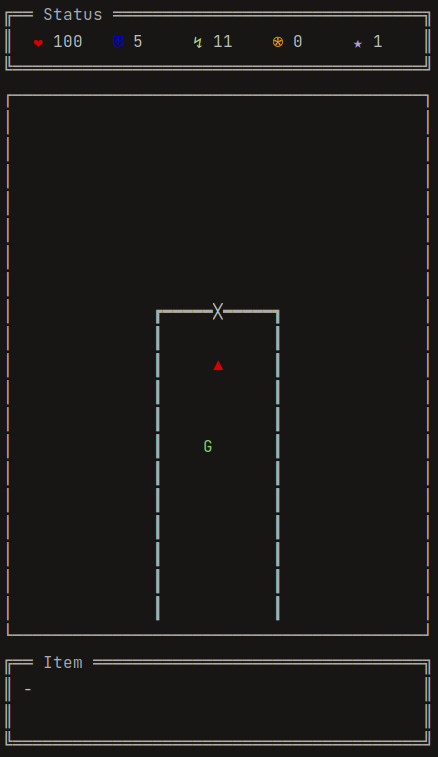
\includegraphics[width=0.6\linewidth]{Bilder/Visualisierung/GameLook.png}
    \caption{Korrekt dargestelltes Konsolen-Interface}
\end{figure}

\section{Wie testet man die Applikation?}
Alle Tests befinden sich im Ordner \texttt{./src/test/java}.
Sie sind mittels \textbf{JUnit5} umgesetzt. Die vorliegenden Tests
können mithilfe der eingebauten IDE-Funktionen einzeln oder im
Verbund ausgeführt werden. Es existieren sowohl
\textit{Blackbox-Integration-Tests}, als auch normale
\textit{Unit Tests}.

\chapter{Clean Architecture}

\section{Was ist Clean Architecture?}
Die \textit{Clean Architecture} ist ein Gestaltungskonzept, das darauf
abzielt möglichst robuste und wartbare Anwendungen zu entwickeln. Dabei
wird eine Software in hierarchisch mehrere Schichten organisiert, was
gemeinhin als \textit{Onion-Architektur} bekannt ist. Jede Schicht
weist dabei eine spezifische Verantwortung (siehe \textit{domain}, 
\textit{plugins} etc.). 

Die Schichten sind über Schnittstellen verbunden. Hinter den
Schnittstellen steckt dann eine tatsächliche Implementation. Ziel ist
es dadurch eine Trennung zwischen der Logik einer Schicht und den
technischen Details einer anliegenden Schicht zu erzeugen. Statt durch
konkrete Implementierungsdetail sind die Schichten (zumindest von innen
nach außen) über
Funktionsabmachungen in Form der Schnittstellen verbunden. Dadurch
lassen sich leicht Änderungen in einer Schicht vornehmen, ohne dabei
zwangsläufig Änderungen in einer anderen Schicht vornehmen zu müssen.

Entscheidend für das Prinzip ist die Abhängigkeitsrichtung. Äußere
abstraktere Schichten (hierarchisch untergeordnet) können direkt auf
innere Schichten zugreifen und von ihnen abhängig sein. Jedoch gilt
dies nicht für die Umkehrrichtung. Aufrufe von innen nach außen werden
über Schnittstellen und Abstraktionen sichergestellt 
(\textit{Dependency Inversion} und \textit{Injection}).
Tieferliegende Schichten sind zudem am wenigsten abstrakt und damit
am langlebigsten.

Dieser Sachverhalt führt zu Anwendungen, die wartbarer und robuster sind,
weil Änderungen an einer Schicht meist keine Änderungen an anderen
Schichten verursachen. Durch clevere Trennung und Abstraktionen lässt
sich der Anpassungaufwand durch eine beliebige Änderung an vielen Stellen
einsparen.

\section{Analyse der Dependency Rule}

\section{Analyse der Schichten}
\chapter{SOLID}

\section{Analyse Single-Responsibility-Principle (SRP)}

\section{Analyse Open-Closed-Principle (OCP)}

\section{Analyse Dependency-Inversion-Principle (DIP)}
\chapter{Weitere Prinzipien}

\section{Analyse GRASP: Geringe Kopplung}
\subsection*{Positiv-Beispiel}
\vspace{0.5cm}
\begin{figure}[H]
    \centering
    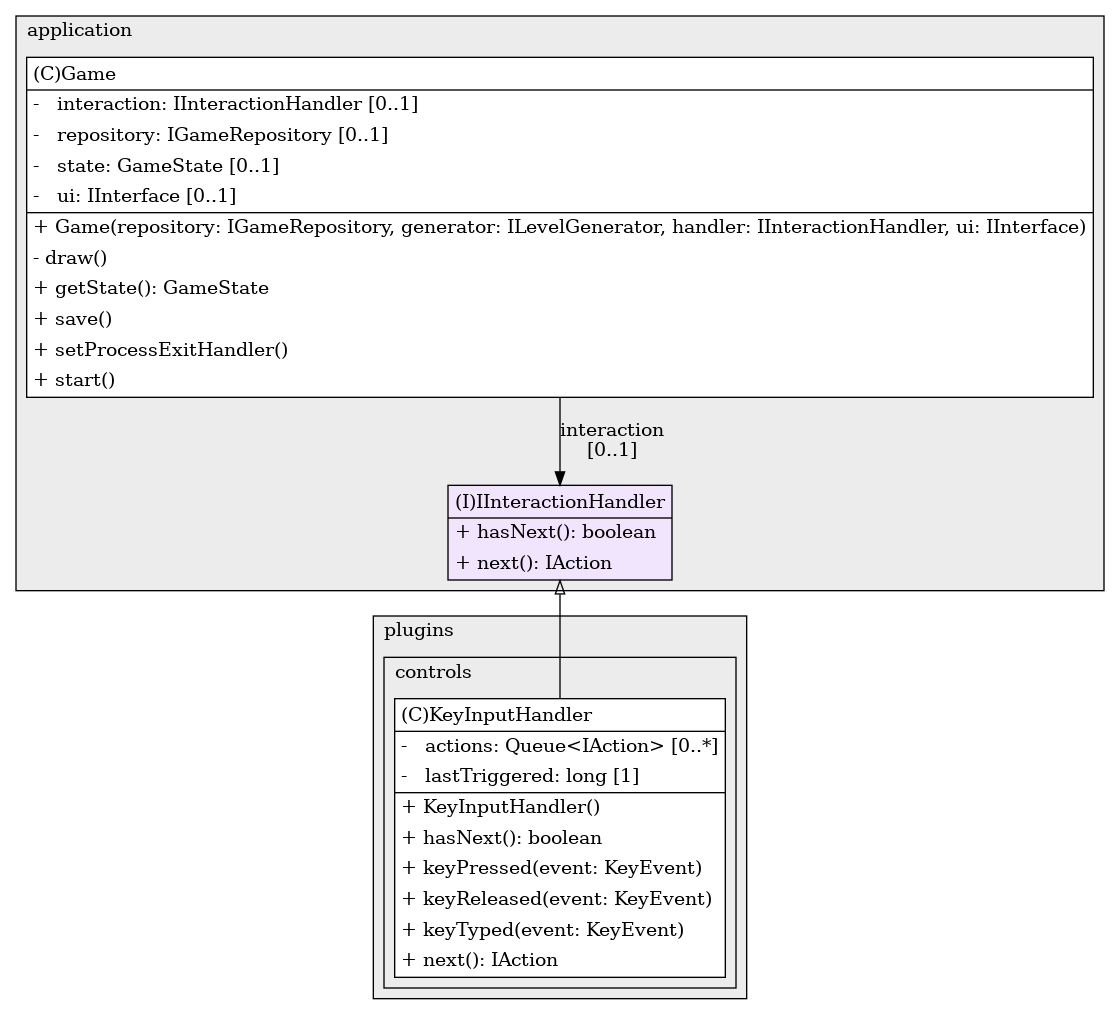
\includegraphics[width=1\linewidth]{Bilder/Visualisierung/IInteractionHandler_structure.png}
    \caption{Analyse GRASP: Geringe Kopplung / Positiv}
\end{figure}

\subsection*{Negativ-Beispiel}
\vspace{0.5cm}
\begin{figure}[H]
    \centering
    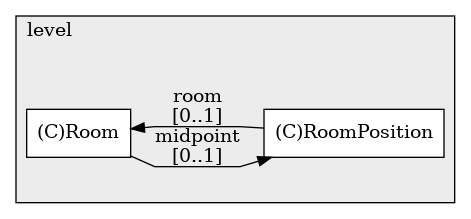
\includegraphics[width=1\linewidth]{Bilder/Visualisierung/RoomPositionNoInterface_structure.png}
    \caption{Analyse GRASP: Geringe Kopplung / Negativ}
\end{figure}

\iffalse
Um die beiden Klassen RoomPosition und Room besser zu entkoppeln, können wir die direkte Abhängigkeit der RoomPosition von der konkreten Room-Implementierung lösen und stattdessen eine abstrakte Schnittstelle oder eine abstrakte Basisklasse einführen. Dadurch wird die Abhängigkeit lockerer und die Klassen können unabhängig voneinander entwickelt, getestet und gewartet werden.

Hier ist ein Beispiel, wie die Klassen entkoppelt werden könnten:

java
Copy code
public interface Room {
    boolean contains(Position position);
    boolean isBlockedByEnemy(Position position);
}

public class ConcreteRoom implements Room {
    // Implementierung der Methoden für den konkreten Raum
    // ...
}

public class RoomPosition extends Position implements IVectorizable {
    private final Room room;

    public RoomPosition(int x, int y, Room room) {
        super(x, y);
        this.room = room;
    }

    public Room getRoom() {
        return this.room;
    }

    public boolean isInside() {
        return this.room.contains(this);
    }

    public boolean isBlockedByEnemy() {
        return this.room.isBlockedByEnemy(this);
    }

    // Restliche Methoden und Implementierung der Klasse
    // ...
}
In diesem Beispiel haben wir die Schnittstelle Room eingeführt, die die benötigten Methoden definiert, die die RoomPosition verwenden möchte. Die konkrete Implementierung ConcreteRoom implementiert diese Schnittstelle und enthält die spezifische Logik für den Raum.

Durch die Verwendung der Schnittstelle Room anstelle der konkreten Room-Klasse wird die Abhängigkeit in der RoomPosition gelockert. Jetzt kann die RoomPosition mit jeder Klasse arbeiten, die die Room-Schnittstelle implementiert, unabhängig von ihrer konkreten Implementierung.

Dies ermöglicht es uns, verschiedene Arten von Räumen zu erstellen und auszutauschen, ohne dass Änderungen an der RoomPosition erforderlich sind. Außerdem erleichtert es das Testen der RoomPosition, da wir Mock-Implementierungen der Room-Schnittstelle verwenden können, um isolierte Tests durchzuführen.

Die Entkopplung der Klassen erhöht die Flexibilität, Wartbarkeit und Testbarkeit des Codes und fördert eine bessere Modulbildung und Wiederverwendbarkeit der Komponenten.

\fi

\section{Analyse GRASP: Hohe Kohäsion}
Das nachfolgende UML-Diagramm zeigt die Klasse \textit{Buffer}, welche
eine sehr hohe Kohäsion aufweist. Sie beschreibt einen Puffer für
Anzeigedaten. Der Puffer enthält sowohl Farb- als auch Zeichendaten
und besitzt eine Größendefinition.

Die Kohäsion ist sehr hoch, weil die Klasse eine einzige
Verantwortlichkeit hat, nämlich die Verwaltung des Puffers. Die
enthaltenen Funktionen sind darüber hinaus lediglich für die 
Manipulation und Anzeige des Pufferinhalts verantwortlich. Sie bilden
verschiedene Manipulationsmethoden ab. Zudem existiert keine externe
Abhängigkeit. Die komplette Logik für die Klasse ist in ihr vereint.

\vspace{0.5cm}
\begin{figure}[H]
    \centering
    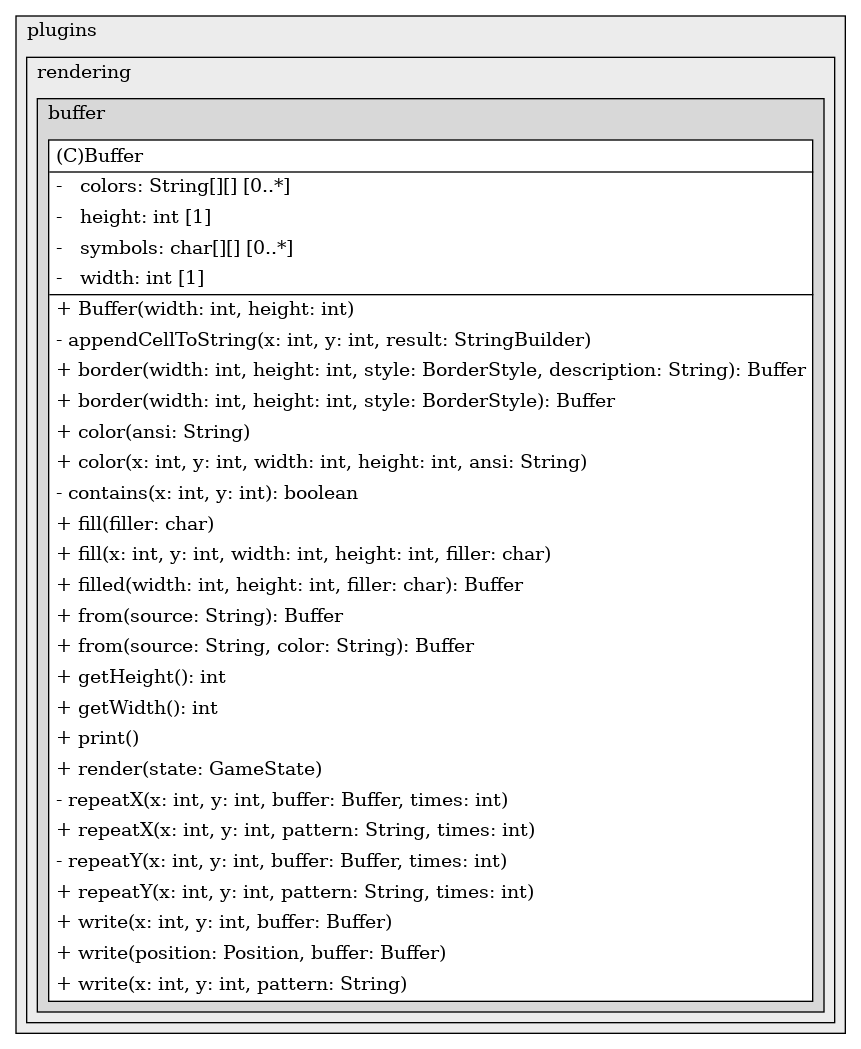
\includegraphics[width=0.75\linewidth]{Bilder/Visualisierung/Buffer_structure.png}
    \caption{Analyse GRASP: Hohe Kohäsion}
\end{figure}

\iffalse
Die gegebene Klasse "Buffer" erfüllt das Kriterium der hohen Kohäsion,
da sie eine klare und spezifische Aufgabe erfüllt, nämlich die
Verwaltung eines Puffers für die Darstellung von Zeichen und Farben.
Hier sind einige Gründe, warum sie hohe Kohäsion aufweist:

Zusammengehörigkeit: Die Methoden und Eigenschaften der Klasse dienen
alle dem Zweck der Pufferverwaltung. Sie ermöglichen das Setzen von
Zeichen und Farben, das Hinzufügen von Inhalten, das Erzeugen von
speziellen Puffern (z. B. mit Rahmen) und die Darstellung des Puffers.

Klare Verantwortlichkeiten: Die Klasse konzentriert sich ausschließlich
auf die Pufferverwaltung und enthält keine Funktionalitäten, die nicht
damit verbunden sind. Sie bietet Methoden zum Setzen von Zeichen,
Farben, zum Schreiben von Inhalten, zum Erzeugen spezieller Puffer und
zur Darstellung des Puffers.

Geringe Abhängigkeit von externen Komponenten: Die Klasse hat keine
Abhängigkeiten von anderen Klassen oder externen Ressourcen. Sie
enthält alle erforderlichen Methoden und Datenstrukturen, um die
Pufferverwaltung durchzuführen.

Einfache Wiederverwendbarkeit: Der Buffer kann in verschiedenen
Anwendungen oder Modulen wiederverwendet werden, in denen eine
Pufferverwaltung erforderlich ist. Die Klasse ist gut isoliert und
unabhängig von anderen Teilen des Systems.

Insgesamt erfüllt die Klasse "Buffer" das Prinzip der hohen Kohäsion,
indem sie eine klare und spezifische Aufgabe erfüllt und ihre Methoden
und Eigenschaften darauf ausgerichtet sind. Dies erleichtert die
Lesbarkeit, Wartbarkeit und Wiederverwendbarkeit des Codes.
\fi

\section{Don't Repeat Yourself (DRY)}

Der erste Code zeigt den Zustand vor der Klassen \textit{Entity},
\textit{Player} und \textit{Goblin} vor der Code-Deduplikation 
(Commit 3d905e1). Tatsächlich waren allerdings noch einige mehr
Klassen auf ähnliche Weise betroffen.

Zu sehen ist, dass die Konstruktor-Funktion von \textit{Entity} nicht
die Möglichkeit bietet alle Felder zu setzen. Diese sind jedoch wichtig
bei der Definition von konkreten Entities, wie \textit{Goblin} oder
\textit{Player}. Daher muss jede Klasse, welche von \textit{Entity}
erbt, die Felder \textit{weapon} und \textit{position} manuell
gesetzt bekommen.

Der zweite Code zeigt, dass die Konstruktor-Funktion entsprechend
erweitert wurde, sodass die Felder nun auch als Argumente entgegengenommen
und an einer zentralen Stelle (\textit{Entity}) entsprechend gesetzt
werden (Commit b125cf0). Damit ist \textit{DRY} erfüllt. Statt
mehrfacher gleicherartiger Wertezuweisungen der Felder in allen
Kindsklassen von \textit{Entity}, geschieht die Zuweisung nur noch an
einer Stelle. 

Zum einen verbessert dies die Komplexität und Wartbarkeit, weil nicht
mehr mehrere Stellen geändert werden müssen, sollte sich z.B. der
Name eines betroffenen Feldes ändern. Zum anderen ist es lesbarer und
weniger fehleranfällig.

\lstset{ 
    language=Java,
    basicstyle=\fontfamily{pcr}\selectfont\footnotesize,
    keywordstyle=\color{purple},
    numberstyle=\tiny,    
    showspaces=false,
    showstringspaces=false,
    showtabs=false, 
    frame=single,
    tabsize=2,
    rulesepcolor=\color{gray},
    rulecolor=\color{black},
    captionpos=b,
    breaklines=true,
    breakatwhitespace=false, 
}

\vspace{0.5cm}
\begin{lstlisting}[caption={Don't Repeat Yourself (Vorher)}]
    public abstract class Entity {
        protected String name;
        protected int health;
        protected Position position;
        protected int baseArmor;
        protected int strength;
        protected Weapon weapon;
     
     
        public Entity(int health, int baseArmor, int strength, String name){
            this.health = health;
            this.baseArmor = baseArmor;
            this.strength = strength;
            this.name = name;
        }
        
        ...
    }     

    public class Player extends Entity {

        public Player(String name) {
            super(100, 5, 10, name);
            weapon = Weapon.FISTS;
            position = new Position(0, 0);
        }


        public String getName() {
            return name;
        }

    }

    public class Goblin extends Entity {
        public Goblin(Position position) {
            super(10, 2, 5, "Goblin");
            weapon = Weapon.DAGGER;
            this.position = position;
        }
    }
\end{lstlisting}

\vspace{0.5cm}
\begin{lstlisting}[caption={Don't Repeat Yourself (Nachher)}]
    public abstract class Entity {
        protected String name;
        protected int health;
        protected Position position;
        protected int baseArmor;
        protected int strength;
        protected Weapon weapon;
     
        public Entity(int health, int baseArmor, int strength, String name, Weapon weapon, Position position){
            this.health = health;
            this.baseArmor = baseArmor;
            this.strength = strength;
            this.name = name;
            this.weapon = weapon;
            this.position = position;
        }
     
        ...
    }

    public class Player extends Entity {

        public Player(String name) {
            super(100, 5, 10, name, Weapon.FISTS, new Position(0,0));
        }

        public String getName() {
            return name;
        }

    }

    public class Goblin extends Entity {

        public Goblin(Position position) {
            super(10, 2, 5, "Goblin", Weapon.DAGGER, position);
        }

    }

\end{lstlisting}
\chapter{Unit Tests}

\section{10 Unit Tests}

\hyphenation{DirectionTest}
\begin{table}[H]
    \centering
    \begin{tabular}{|p{8cm}|p{8cm}|}
      \hline
      \textbf{Unit Test} & \textbf{Beschreibung} \\
      \hline
      1. VectorTest\#dotTest & Testet \textit{dotTest}-Funktion der Klasse \textit{Vector} darauf, ob sie korrekt Skalarprodukte berechnet \\
      \hline
      2. VectorTest\#lengthTest & Testet \textit{length}-Funktion der Klasse \textit{Vector} darauf, ob sie korrekt Vektorlängen berechnet \\
      \hline
      3. VectorTest\#getClockwiseAngleFromTest & Testet \textit{getClockwiseAngleFrom}-Funktion der Klasse \textit{Vector} darauf, ob sie korrekt Winkel zwischen zwei Vektoren berechnet \\
      \hline
      4. NumericTest\#clampTest & Testet \textit{clamp}-Funktion der Klasse \textit{Numeric} darauf, ob sie korrekt Werte in einem gegebenen Interval einschließt \\
      \hline
      5. EntityTest\#getPreferredMovement DirectionTest & Testet \textit{getPreferredMovementDirection}-Funktion der Klasse \textit{Enemy} darauf, ob sie korrekt eine Bewegung aufgrund der Position des Spielers wählt \\
      \hline
      6. RoomGridTest\#fitsTest & Testet \textit{fits}-Funktion der Klasse \textit{RoomGrid} darauf, ob sie korrekt feststellen kann, ob ein Raum noch auf die Spielkarte passt \\
      \hline
      7. RoomPositionTest\#getMaxDistanceAlongAnyAxisTest & Testet \textit{getMaxDistanceAlongAnyAxis}-Funktion der Klasse \textit{RoomPosition} darauf, ob sie korrekt die maximale Entfernung entlang einer von beiden Axen von einem Punkt zum anderen berechnen kann \\
      \hline
      8. CollectionSelectorTest\#randomSubset Test & Testet \textit{random}-Funktion der Klasse \textit{CollectionSelector} darauf, ob sie korrekt Teilmengen der Auswahl selektiert \\
      \hline
    \end{tabular}
    \caption{Unit Tests mit Beschreibung I}
\end{table}

\begin{table}[H]
    \centering
    \begin{tabular}{|p{8cm}|p{8cm}|}
      \hline
      \textbf{Unit Test} & \textbf{Beschreibung} \\
      \hline
      9. GameStateTest\#movementTest & Testet \textit{dotTest}-Funktion der Klasse \textit{Vector} darauf, ob sie korrekt Skalarprodukte berechnet \\
      \hline
      10. VectorTest\#lengthTest & Testet \textit{length}-Funktion der Klasse \textit{Vector} darauf, ob sie korrekt Vektorlängen berechnet \\
      \hline
    \end{tabular}
    \caption{Unit Tests mit Beschreibung II}
\end{table}

\section{ATRIP: Automatic}
Der Begriff \textit{Automatic} bezieht sich auf die automatische
Ausführung von Unit Tests. Dies kann mit herkömmlichen Test-Frameworks
wie etwa \textit{JUnit5} erreicht werden. 

Dabei können Methoden eigens zum Testen erstellt werden, welche mit
\textit{@Test} annotiert werden. Innerhalb der IDE (z.B. IntelliJ)
können sie dann über einen Befehl oder Knopfdruck einzeln oder im
Gesamten ausgeführt werden.

Die Tests sind so konzipiert, dass sie nicht andere Durchläufe beeinflussen.
Sie sind also unabhängig von einander (\textit{Independence}) und 
wiederholbar (\textit{Repeatability}). Das führt zu nachvollziehbaren
Ergebnissen. Zudem besitzen die Tests keine externen Abhängigkeiten.

Zum Schluss gibt JUnit eine Zusammenfassung aus. Diese beschreibt die
erfolgreichen und fehlgeschlagenen Tests.

\section{ATRIP: Thorough}
\subsection*{Positiv-Beispiel}
Der nachfolgende Code-Ausschnitt zeigt das Positiv-Beispiel zum
\textit{Thorough}-Aspekt. Hierbei wird die
\textit{getClockwiseAngleFromTest()}-Funktion der Klasse
\textit{Vector} getestet, welche den Winkel im Uhrzeigersinn 
zwischen zwei Vektoren berechnet. Dabei gibt es einige verschiedene
Möglichkeiten. Diese hängen unter anderem von der Definitionsreihenfolge
der beiden involvierten Vektoren ab. Dabei beginnt die Winkelmessung
beim zweiten angegebenen Vektor und läuft bis zum ersten Vektor im
Uhrzeigersinn. Es gibt zudem auch Fälle, in denen die Berechnung
fehlschlägt, etwa dann wenn ein Vektor der Nullvektor ist.

Der Test ist \textit{Thorough}, da er als \textit{ParameterizedTest}
umgesetzt ist und die Eingabe-Quelle \textit{getClockwiseAngleFromArguments()}
eine gründliche Stichprobe möglicher Fälle bereitstellt. Dabei werden
etwa Standardfälle in einigen Ausführungen und Definitionsreihenfolgen
ausprobiert, sowie unübliche Fälle, Edge Cases und pathologische Fälle.

\lstset{ 
    language=Java,
    basicstyle=\fontfamily{pcr}\selectfont\footnotesize,
    keywordstyle=\color{purple},
    numberstyle=\tiny,    
    showspaces=false,
    showstringspaces=false,
    showtabs=false, 
    frame=single,
    tabsize=2,
    rulesepcolor=\color{gray},
    rulecolor=\color{black},
    captionpos=b,
    breaklines=true,
    breakatwhitespace=false, 
}

\vspace{1cm}
\begin{lstlisting}[caption={ATRIP: Thorough / Positiv}]
    @ParameterizedTest
    @MethodSource("getClockwiseAngleFromArguments")
    void getClockwiseAngleFromTest(Vector to, Vector from, double angle) {
        assertEquals(angle, to.getClockwiseAngleFrom(from));
    }
    
    private static List<Arguments> getClockwiseAngleFromArguments() {
        return List.of(
                Arguments.of(Vector.UP, Vector.UP, 0D),
                Arguments.of(Vector.RIGHT, Vector.UP, 90D),
                Arguments.of(Vector.UP, Vector.RIGHT, 270D),
                Arguments.of(Vector.LEFT, Vector.UP, 270D),
                Arguments.of(Vector.UP, Vector.LEFT, 90D),
                Arguments.of(Vector.DOWN, Vector.UP, 180D),
                Arguments.of(Vector.UP, Vector.DOWN, 180D),
                
                Arguments.of(new Vector(1, 2), new Vector(1, 2), 0D),
                Arguments.of(new Vector(1, 1), new Vector(1, -1), 90D),
                Arguments.of(new Vector(-1, 1), new Vector(1, -1), 180D),
                
                Arguments.of(new Vector(1, 1), Vector.RIGHT, 45D),
                Arguments.of(new Vector(10000, 0), Vector.UP, 90D),
                
                Arguments.of(new Vector(0, 0), Vector.UP, Double.NEGATIVE_INFINITY),
                Arguments.of(new Vector(0, 0), Vector.RIGHT, Double.NEGATIVE_INFINITY)
        );
    }
\end{lstlisting}

\subsection*{Negativ-Beispiel}

\section{ATRIP: Professional}

\section{Code Coverage}

\section{Fakes und Mocks}
\chapter{Domain Driven Design}

\section{Ubiquitous Language (UL)}
\subsection*{Item}

\textbf{Bedeutung}: Ein \textit{Item} ist ein nicht-belebtes Objekt,
welches einen konkreten Gegendstand im Spiel wie etwa Waffen,
Rüstungen oder Münzen repräsentiert. Mit ihm kann interagiert werden.
Ein Item erfüllt verschiedene Funktionen abhängig vom Typ, wie etwa
Heilung, Stärkung des Spielers oder Beeinflussung des Spielstandes.

\textbf{Begründung}: Die Verwendung des Begriffes in der UL erlaubt
eine einheitliche Kommunikation zwischen den Entwicklern und Designern.
Hinzu kommt, dass der Begriff grundlegend in der Spieleentwicklung ist.
Somit lässt sich leichter festlegen, wie Items designed und logisch
in das Spielgeschehen integriert werden und wie diese die Spielerfahrung
formen.



\subsection*{Room}

\textbf{Bedeutung}: Der Begriff \textit{Room} definiert einen
abgegrenzten Bereich der Spielwelt. Jeder Raum stellt für den Spieler
eine neue Herausforderung dar. In ihm befinden sich neue Gegner und
neue Items. Besonders ersichtlich wird die Abgrenzung der Räume, wenn
sie abgeschlossen sind, weil in ihnen noch Gegner leben.

\textbf{Begründung}: Der Begriff Room in der UL ist essentiell wichtig,
da Entwickler und Designer sich absprechen müssen, um den technischen
und stilistischen Entwurf für abgegrenze Spielbereiche zu schaffen.
Für Entwickler ist der Begriff besonders prägend im Bereich der Welt-
Generierung. Für Designer ist er wichtig, um zwischen verschiedenen
Typen zu unterscheiden, welche unterschiedlich ausgebildet werden.



\subsection*{Level}

\textbf{Bedeutung}: Das \textit{Level} repräsentiert eine abgegrenzte
Spielstufe. Es gilt dieses komplett zu absolvieren, bis man den
End-Raum des Levels gefunden hat. Es stellt eine Einheit einzelner mit
einander verbundener Räume dar. Levels haben Fortschrittsmechanismen
bezogen auf die Schwierigkeit der Räume.

\textbf{Begründung}: Der Begriff \textit{Level} ist in der UL sehr
wichtig, da es einen Strukturbegriff darstellt. Er gliedert die
Spielwelt weiter als übergeordneter Einheit über den Räumen. Daher
ist der Begriff relevant für Entwickler im Bezug auf die Welt-Generierung
und für Designer im Bezug auf die Schwierigkeitsentwicklung und den
Stil.



\subsection*{Player}

\textbf{Bedeutung}: Der \textit{Player} stellt die Spielfigur dar,
durch welche der Spielende mit der virtuellen Umgebung interagieren
kann. Er stellt ein sterbliches Lebewesen dar, welches den Umgang mit
der Spielwelt maßgeblich beeinflusst: Das oberste Ziel ist überleben.
Der Spieler kann Items aufsammeln, Gegnern schaden zufügen, von ihnen
Schaden nehmen und durch die Räume gehen.

\textbf{Begründung}: Die Verwendung des Begriffs \textit{Player}
schafft Klarheit in der Abgrenzung zu anderen virtuellen Lebewesen
wie den Gegnern. Der Spieler hat eine gesonderte Rolle und benötigt
daher wesentlichen Mehraufwand in der Entwicklung und Design. Seine
Interaktionen prägen das Spielerlebnis. Technisch gesehen teilt sich
ein Spieler Eigenschaften mit anderen Lebewesen. Daher ist eine klare
Definition der Spielfigur unerlässlich für die Entwicklung selbst, um
die herausstellenden Merkmale klar abzugrenzen.

\section{Entities}

\section{Value Objects}

\section{Repositories}

\section{Aggregates}
\chapter{Refactoring}

\section{Code Smells}

\subsection*{}
\vspace{0.5cm}
\begin{lstlisting}[caption={Code Smell I (Vorher)}]
    @Override
    public void move(Direction direction) {
        RoomPosition target = this.getPosition().getAdjacentPosition(direction);
        if (target.isValid() && target.isFree()) {
            if (this.getRoom() instanceof BossRoom boss) {
                RoomPosition trapdoor = boss.getTrapdoorPosition();
                
                if (target.equals(trapdoor) && this.getRoom().isCleared()) {
                    this.game.nextLevel();
                }
            }
            
            this.setPosition(target);
            
            Item underneath = this.getRoom().getItemUnderneath(this.getPosition());
            // this.game.setItemUnderneath(underneath);
        } else {
            if (!this.getRoom().isCleared()) {
                return;
            }
            
            this.getRoom().getDoors().forEach(door -> {
                if (door.getRoomPosition().equals(target)) {
                    this.game.getLevel().enter(door);
                }
            });
        }
    }
\end{lstlisting}

\vspace{0.5cm}
\begin{lstlisting}[caption={Code Smell I (Nachher)}]
    @Override
    public void move(Direction direction) {
        RoomPosition target = this.getPosition().getAdjacentPosition(direction);
        if (target.isValid() && target.isFree()) {
            if (this.getRoom().isBossRoom()) {
                RoomPosition trapdoor = this.getRoom().getTrapdoorPosition();
                if (target.equals(trapdoor) && this.getRoom().isCleared()) {
                    this.game.nextLevel();
                }
            }
            
            this.setPosition(target);
            
            Item underneath = this.getRoom().getItemAt(this.getPosition());
            // this.game.setItemUnderneath(underneath);
        } else {
            if (!this.getRoom().isCleared()) {
                return;
            }
            
            Door door = this.getRoom().getDoorAt(target);
            if (door != null) {
                this.game.getLevel().enter(door);
            }
        }
    }
\end{lstlisting}


\section{Refactorings}
\chapter{Entwurfsmuster}

\section{Entwurfsmuster: Fabrik}

\section{Entwurfsmuster: Kompositum}

% ---- Literaturverzeichnis
\cleardoublepage
\renewcommand*{\chapterpagestyle}{plain}
\pagestyle{plain}
\pagenumbering{Roman}                   % Römische Seitenzahlen
\setcounter{page}{\numexpr\value{savepage}+1}
%\printbibliography[title=References]

% ---- Anhang
\appendix 
\clearpage
\pagenumbering{Roman}  % römische Seitenzahlen für Anhang

\newpage
\end{document}
